<<<<<<< HEAD
\documentclass[]{article}
\usepackage{lmodern}
\usepackage{amssymb,amsmath}
\usepackage{ifxetex,ifluatex}
\usepackage{fixltx2e} % provides \textsubscript
\ifnum 0\ifxetex 1\fi\ifluatex 1\fi=0 % if pdftex
  \usepackage[T1]{fontenc}
  \usepackage[utf8]{inputenc}
\else % if luatex or xelatex
  \ifxetex
    \usepackage{mathspec}
  \else
    \usepackage{fontspec}
  \fi
  \defaultfontfeatures{Ligatures=TeX,Scale=MatchLowercase}
    \setmainfont[]{NanumGothic}
\fi
% use upquote if available, for straight quotes in verbatim environments
\IfFileExists{upquote.sty}{\usepackage{upquote}}{}
% use microtype if available
\IfFileExists{microtype.sty}{%
\usepackage{microtype}
\UseMicrotypeSet[protrusion]{basicmath} % disable protrusion for tt fonts
}{}
\usepackage[margin=1in]{geometry}
\usepackage{hyperref}
\hypersetup{unicode=true,
            pdftitle={hw7\_Clustering},
            pdfauthor={201511646\_나여영},
            pdfborder={0 0 0},
            breaklinks=true}
\urlstyle{same}  % don't use monospace font for urls
\usepackage{color}
\usepackage{fancyvrb}
\newcommand{\VerbBar}{|}
\newcommand{\VERB}{\Verb[commandchars=\\\{\}]}
\DefineVerbatimEnvironment{Highlighting}{Verbatim}{commandchars=\\\{\}}
% Add ',fontsize=\small' for more characters per line
\usepackage{framed}
\definecolor{shadecolor}{RGB}{248,248,248}
\newenvironment{Shaded}{\begin{snugshade}}{\end{snugshade}}
\newcommand{\KeywordTok}[1]{\textcolor[rgb]{0.13,0.29,0.53}{\textbf{{#1}}}}
\newcommand{\DataTypeTok}[1]{\textcolor[rgb]{0.13,0.29,0.53}{{#1}}}
\newcommand{\DecValTok}[1]{\textcolor[rgb]{0.00,0.00,0.81}{{#1}}}
\newcommand{\BaseNTok}[1]{\textcolor[rgb]{0.00,0.00,0.81}{{#1}}}
\newcommand{\FloatTok}[1]{\textcolor[rgb]{0.00,0.00,0.81}{{#1}}}
\newcommand{\ConstantTok}[1]{\textcolor[rgb]{0.00,0.00,0.00}{{#1}}}
\newcommand{\CharTok}[1]{\textcolor[rgb]{0.31,0.60,0.02}{{#1}}}
\newcommand{\SpecialCharTok}[1]{\textcolor[rgb]{0.00,0.00,0.00}{{#1}}}
\newcommand{\StringTok}[1]{\textcolor[rgb]{0.31,0.60,0.02}{{#1}}}
\newcommand{\VerbatimStringTok}[1]{\textcolor[rgb]{0.31,0.60,0.02}{{#1}}}
\newcommand{\SpecialStringTok}[1]{\textcolor[rgb]{0.31,0.60,0.02}{{#1}}}
\newcommand{\ImportTok}[1]{{#1}}
\newcommand{\CommentTok}[1]{\textcolor[rgb]{0.56,0.35,0.01}{\textit{{#1}}}}
\newcommand{\DocumentationTok}[1]{\textcolor[rgb]{0.56,0.35,0.01}{\textbf{\textit{{#1}}}}}
\newcommand{\AnnotationTok}[1]{\textcolor[rgb]{0.56,0.35,0.01}{\textbf{\textit{{#1}}}}}
\newcommand{\CommentVarTok}[1]{\textcolor[rgb]{0.56,0.35,0.01}{\textbf{\textit{{#1}}}}}
\newcommand{\OtherTok}[1]{\textcolor[rgb]{0.56,0.35,0.01}{{#1}}}
\newcommand{\FunctionTok}[1]{\textcolor[rgb]{0.00,0.00,0.00}{{#1}}}
\newcommand{\VariableTok}[1]{\textcolor[rgb]{0.00,0.00,0.00}{{#1}}}
\newcommand{\ControlFlowTok}[1]{\textcolor[rgb]{0.13,0.29,0.53}{\textbf{{#1}}}}
\newcommand{\OperatorTok}[1]{\textcolor[rgb]{0.81,0.36,0.00}{\textbf{{#1}}}}
\newcommand{\BuiltInTok}[1]{{#1}}
\newcommand{\ExtensionTok}[1]{{#1}}
\newcommand{\PreprocessorTok}[1]{\textcolor[rgb]{0.56,0.35,0.01}{\textit{{#1}}}}
\newcommand{\AttributeTok}[1]{\textcolor[rgb]{0.77,0.63,0.00}{{#1}}}
\newcommand{\RegionMarkerTok}[1]{{#1}}
\newcommand{\InformationTok}[1]{\textcolor[rgb]{0.56,0.35,0.01}{\textbf{\textit{{#1}}}}}
\newcommand{\WarningTok}[1]{\textcolor[rgb]{0.56,0.35,0.01}{\textbf{\textit{{#1}}}}}
\newcommand{\AlertTok}[1]{\textcolor[rgb]{0.94,0.16,0.16}{{#1}}}
\newcommand{\ErrorTok}[1]{\textcolor[rgb]{0.64,0.00,0.00}{\textbf{{#1}}}}
\newcommand{\NormalTok}[1]{{#1}}
\usepackage{graphicx,grffile}
\makeatletter
\def\maxwidth{\ifdim\Gin@nat@width>\linewidth\linewidth\else\Gin@nat@width\fi}
\def\maxheight{\ifdim\Gin@nat@height>\textheight\textheight\else\Gin@nat@height\fi}
\makeatother
% Scale images if necessary, so that they will not overflow the page
% margins by default, and it is still possible to overwrite the defaults
% using explicit options in \includegraphics[width, height, ...]{}
\setkeys{Gin}{width=\maxwidth,height=\maxheight,keepaspectratio}
\IfFileExists{parskip.sty}{%
\usepackage{parskip}
}{% else
\setlength{\parindent}{0pt}
\setlength{\parskip}{6pt plus 2pt minus 1pt}
}
\setlength{\emergencystretch}{3em}  % prevent overfull lines
\providecommand{\tightlist}{%
  \setlength{\itemsep}{0pt}\setlength{\parskip}{0pt}}
\setcounter{secnumdepth}{0}
% Redefines (sub)paragraphs to behave more like sections
\ifx\paragraph\undefined\else
\let\oldparagraph\paragraph
\renewcommand{\paragraph}[1]{\oldparagraph{#1}\mbox{}}
\fi
\ifx\subparagraph\undefined\else
\let\oldsubparagraph\subparagraph
\renewcommand{\subparagraph}[1]{\oldsubparagraph{#1}\mbox{}}
\fi

%%% Use protect on footnotes to avoid problems with footnotes in titles
\let\rmarkdownfootnote\footnote%
\def\footnote{\protect\rmarkdownfootnote}

%%% Change title format to be more compact
\usepackage{titling}

% Create subtitle command for use in maketitle
\newcommand{\subtitle}[1]{
  \posttitle{
    \begin{center}\large#1\end{center}
    }
}

\setlength{\droptitle}{-2em}
  \title{hw7\_Clustering}
  \pretitle{\vspace{\droptitle}\centering\huge}
  \posttitle{\par}
  \author{201511646\_나여영}
  \preauthor{\centering\large\emph}
  \postauthor{\par}
  \predate{\centering\large\emph}
  \postdate{\par}
  \date{2017년 11월 27일}


\begin{document}
\maketitle

\subsection{HW7\_Clustering\_201511646}\label{hw7_clustering_201511646}

\begin{quote}
\begin{enumerate}
\def\labelenumi{\arabic{enumi}.}
\tightlist
\item
  In this example, we have distances between ten American cities based
  on the flying mileages between them. The objective is to see if we can
  define clusters of these cities based on the distances.
\end{enumerate}
\end{quote}

\begin{Shaded}
\begin{Highlighting}[]
\NormalTok{Atlanta<-}\KeywordTok{c}\NormalTok{(}\DecValTok{0}\NormalTok{,}\DecValTok{587}\NormalTok{,}\DecValTok{1212}\NormalTok{,}\DecValTok{701}\NormalTok{,}\DecValTok{1936}\NormalTok{,}\DecValTok{604}\NormalTok{,}\DecValTok{748}\NormalTok{,}\DecValTok{2139}\NormalTok{,}\DecValTok{2182}\NormalTok{,}\DecValTok{543}\NormalTok{)}
\NormalTok{Chicago<-}\KeywordTok{c}\NormalTok{(}\DecValTok{587}\NormalTok{,}\DecValTok{0}\NormalTok{,}\DecValTok{920}\NormalTok{,}\DecValTok{940}\NormalTok{,}\DecValTok{1745}\NormalTok{,}\DecValTok{1188}\NormalTok{,}\DecValTok{713}\NormalTok{,}\DecValTok{1858}\NormalTok{,}\DecValTok{1737}\NormalTok{,}\DecValTok{597}\NormalTok{)}
\NormalTok{Denver<-}\KeywordTok{c}\NormalTok{(}\DecValTok{1212}\NormalTok{,}\DecValTok{920}\NormalTok{,}\DecValTok{0}\NormalTok{,}\DecValTok{879}\NormalTok{,}\DecValTok{831}\NormalTok{,}\DecValTok{1726}\NormalTok{,}\DecValTok{1631}\NormalTok{,}\DecValTok{949}\NormalTok{,}\DecValTok{1021}\NormalTok{,}\DecValTok{1494}\NormalTok{)}
\NormalTok{Houston<-}\KeywordTok{c}\NormalTok{(}\DecValTok{701}\NormalTok{,}\DecValTok{940}\NormalTok{,}\DecValTok{879}\NormalTok{,}\DecValTok{0}\NormalTok{,}\DecValTok{1374}\NormalTok{,}\DecValTok{968}\NormalTok{,}\DecValTok{1420}\NormalTok{,}\DecValTok{1645}\NormalTok{,}\DecValTok{1891}\NormalTok{,}\DecValTok{1220}\NormalTok{)}
\NormalTok{LA<-}\KeywordTok{c}\NormalTok{(}\DecValTok{1936}\NormalTok{,}\DecValTok{1745}\NormalTok{,}\DecValTok{831}\NormalTok{,}\DecValTok{1374}\NormalTok{,}\DecValTok{0}\NormalTok{,}\DecValTok{2339}\NormalTok{,}\DecValTok{2451}\NormalTok{,}\DecValTok{347}\NormalTok{,}\DecValTok{959}\NormalTok{,}\DecValTok{2300}\NormalTok{)}
\NormalTok{Miami<-}\KeywordTok{c}\NormalTok{(}\DecValTok{604}\NormalTok{,}\DecValTok{1188}\NormalTok{,}\DecValTok{1726}\NormalTok{,}\DecValTok{968}\NormalTok{,}\DecValTok{2339}\NormalTok{,}\DecValTok{0}\NormalTok{,}\DecValTok{1092}\NormalTok{,}\DecValTok{2594}\NormalTok{,}\DecValTok{2734}\NormalTok{,}\DecValTok{923}\NormalTok{)}
\NormalTok{Newyork<-}\KeywordTok{c}\NormalTok{(}\DecValTok{748}\NormalTok{,}\DecValTok{713}\NormalTok{,}\DecValTok{1631}\NormalTok{,}\DecValTok{1420}\NormalTok{,}\DecValTok{2451}\NormalTok{,}\DecValTok{1092}\NormalTok{,}\DecValTok{0}\NormalTok{,}\DecValTok{2571}\NormalTok{,}\DecValTok{2408}\NormalTok{,}\DecValTok{205}\NormalTok{)}
\NormalTok{Sanfrancisco<-}\KeywordTok{c}\NormalTok{(}\DecValTok{2139}\NormalTok{,}\DecValTok{1858}\NormalTok{,}\DecValTok{949}\NormalTok{,}\DecValTok{1645}\NormalTok{,}\DecValTok{347}\NormalTok{,}\DecValTok{2594}\NormalTok{,}\DecValTok{2571}\NormalTok{,}\DecValTok{0}\NormalTok{,}\DecValTok{678}\NormalTok{,}\DecValTok{2442}\NormalTok{)}
\NormalTok{Seattle<-}\KeywordTok{c}\NormalTok{(}\DecValTok{2182}\NormalTok{,}\DecValTok{1737}\NormalTok{,}\DecValTok{1021}\NormalTok{,}\DecValTok{1891}\NormalTok{,}\DecValTok{959}\NormalTok{,}\DecValTok{2734}\NormalTok{,}\DecValTok{2408}\NormalTok{,}\DecValTok{678}\NormalTok{,}\DecValTok{0}\NormalTok{,}\DecValTok{2329}\NormalTok{)}
\NormalTok{WashingtonDC<-}\KeywordTok{c}\NormalTok{(}\DecValTok{543}\NormalTok{,}\DecValTok{597}\NormalTok{,}\DecValTok{1494}\NormalTok{,}\DecValTok{1220}\NormalTok{,}\DecValTok{2300}\NormalTok{,}\DecValTok{923}\NormalTok{,}\DecValTok{205}\NormalTok{,}\DecValTok{2442}\NormalTok{,}\DecValTok{2329}\NormalTok{,}\DecValTok{0}\NormalTok{)}
\end{Highlighting}
\end{Shaded}

다음은 대칭행렬이 맞는지 확인하는 과정이다

\begin{Shaded}
\begin{Highlighting}[]
\NormalTok{cities<-}\KeywordTok{matrix}\NormalTok{(}\KeywordTok{c}\NormalTok{(Atlanta,Chicago,Denver, Houston,LA, Miami, Newyork,Sanfrancisco, Seattle, WashingtonDC),}\DecValTok{10}\NormalTok{,}\DataTypeTok{byrow=}\NormalTok{T)}
\NormalTok{cities}
\end{Highlighting}
\end{Shaded}

\begin{verbatim}
##       [,1] [,2] [,3] [,4] [,5] [,6] [,7] [,8] [,9] [,10]
##  [1,]    0  587 1212  701 1936  604  748 2139 2182   543
##  [2,]  587    0  920  940 1745 1188  713 1858 1737   597
##  [3,] 1212  920    0  879  831 1726 1631  949 1021  1494
##  [4,]  701  940  879    0 1374  968 1420 1645 1891  1220
##  [5,] 1936 1745  831 1374    0 2339 2451  347  959  2300
##  [6,]  604 1188 1726  968 2339    0 1092 2594 2734   923
##  [7,]  748  713 1631 1420 2451 1092    0 2571 2408   205
##  [8,] 2139 1858  949 1645  347 2594 2571    0  678  2442
##  [9,] 2182 1737 1021 1891  959 2734 2408  678    0  2329
## [10,]  543  597 1494 1220 2300  923  205 2442 2329     0
\end{verbatim}

\begin{Shaded}
\begin{Highlighting}[]
\NormalTok{Tcities=}\KeywordTok{t}\NormalTok{(cities)}

\KeywordTok{library}\NormalTok{(dplyr)}
\end{Highlighting}
\end{Shaded}

\begin{verbatim}
## Warning: package 'dplyr' was built under R version 3.4.2
\end{verbatim}

\begin{verbatim}
## 
## Attaching package: 'dplyr'
\end{verbatim}

\begin{verbatim}
## The following objects are masked from 'package:stats':
## 
##     filter, lag
\end{verbatim}

\begin{verbatim}
## The following objects are masked from 'package:base':
## 
##     intersect, setdiff, setequal, union
\end{verbatim}

\begin{Shaded}
\begin{Highlighting}[]
\KeywordTok{all_equal}\NormalTok{(cities, Tcities)}
\end{Highlighting}
\end{Shaded}

\begin{verbatim}
## [1] TRUE
\end{verbatim}

맞는지 확인했으므로 그 후 scatter plot을 확인해 데이터의 분포를 본다.

\begin{Shaded}
\begin{Highlighting}[]
\KeywordTok{colnames}\NormalTok{(cities)<-}\KeywordTok{c}\NormalTok{(}\StringTok{"Atlanta"}\NormalTok{,}\StringTok{"Chicago"}\NormalTok{,}\StringTok{"Denver"}\NormalTok{, }\StringTok{"Houston"}\NormalTok{,}\StringTok{"LA"}\NormalTok{, }\StringTok{"Miami"}\NormalTok{, }\StringTok{"Newyork"}\NormalTok{,}\StringTok{"Sanfrancisco"}\NormalTok{, }\StringTok{"Seattle"}\NormalTok{, }\StringTok{"WashingtonDC"}\NormalTok{)}
\KeywordTok{rownames}\NormalTok{(cities)<-}\KeywordTok{c}\NormalTok{(}\StringTok{"Atlanta"}\NormalTok{,}\StringTok{"Chicago"}\NormalTok{,}\StringTok{"Denver"}\NormalTok{, }\StringTok{"Houston"}\NormalTok{,}\StringTok{"LA"}\NormalTok{, }\StringTok{"Miami"}\NormalTok{, }\StringTok{"Newyork"}\NormalTok{,}\StringTok{"Sanfrancisco"}\NormalTok{, }\StringTok{"Seattle"}\NormalTok{, }\StringTok{"WashingtonDC"}\NormalTok{)}

\KeywordTok{plot}\NormalTok{(cities,}\DataTypeTok{pch =} \DecValTok{19}\NormalTok{, }\DataTypeTok{xlab =} \KeywordTok{c}\NormalTok{(}\StringTok{"x coordinate"}\NormalTok{), }\DataTypeTok{ylab =} \KeywordTok{c}\NormalTok{(}\StringTok{"y coordinate"}\NormalTok{),}\DataTypeTok{main =} \StringTok{"Scatter plot of Cities"}\NormalTok{)}
\KeywordTok{text}\NormalTok{(cities, }\DataTypeTok{labels =} \KeywordTok{abbreviate}\NormalTok{(}\KeywordTok{colnames}\NormalTok{(cities)), }\DataTypeTok{cex =} \FloatTok{0.8}\NormalTok{, }\DataTypeTok{pos =} \DecValTok{3}\NormalTok{, }\DataTypeTok{col =} \StringTok{"blue"}\NormalTok{) }\CommentTok{# pos=1 : at the bottom}
\end{Highlighting}
\end{Shaded}

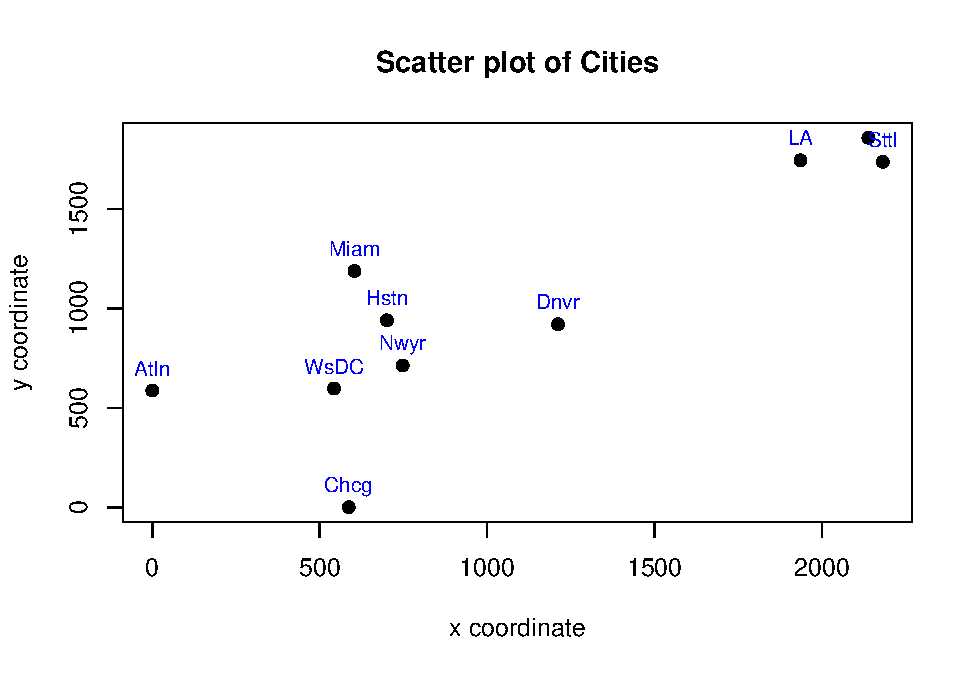
\includegraphics{hw7_files/figure-latex/unnamed-chunk-3-1.pdf}

\begin{quote}
\begin{enumerate}
\def\labelenumi{\arabic{enumi})}
\tightlist
\item
  Do the cluster analysis using (1) single linkage, (2) average linkage
  and (3) the centroid method.
\end{enumerate}
\end{quote}

(1)single linkage

\begin{Shaded}
\begin{Highlighting}[]
\NormalTok{hc1_cities<-}\KeywordTok{hclust}\NormalTok{(}\KeywordTok{dist}\NormalTok{(cities, }\DataTypeTok{method=}\StringTok{"euclidian"}\NormalTok{)^}\DecValTok{2}\NormalTok{, }\DataTypeTok{method=}\StringTok{"single"}\NormalTok{)}
\NormalTok{hc1_cities}
\end{Highlighting}
\end{Shaded}

\begin{verbatim}
## 
## Call:
## hclust(d = dist(cities, method = "euclidian")^2, method = "single")
## 
## Cluster method   : single 
## Distance         : euclidean 
## Number of objects: 10
\end{verbatim}

\begin{Shaded}
\begin{Highlighting}[]
\KeywordTok{rev}\NormalTok{(hc1_cities) }\CommentTok{#height : 군집간 거리 / merge: 병합순}
\end{Highlighting}
\end{Shaded}

\begin{verbatim}
## $dist.method
## [1] "euclidean"
## 
## $call
## hclust(d = dist(cities, method = "euclidian")^2, method = "single")
## 
## $method
## [1] "single"
## 
## $labels
##  [1] "Atlanta"      "Chicago"      "Denver"       "Houston"     
##  [5] "LA"           "Miami"        "Newyork"      "Sanfrancisco"
##  [9] "Seattle"      "WashingtonDC"
## 
## $order
##  [1]  9  5  8  3  4  6  7 10  1  2
## 
## $height
## [1]  272544  560711 1435040 1490187 1581207 2363192 2905270 4037129 4895001
## 
## $merge
##       [,1] [,2]
##  [1,]   -7  -10
##  [2,]   -5   -8
##  [3,]   -9    2
##  [4,]   -1   -2
##  [5,]    1    4
##  [6,]   -6    5
##  [7,]   -4    6
##  [8,]   -3    7
##  [9,]    3    8
\end{verbatim}


\end{document}
=======
\documentclass[]{article}
\usepackage{lmodern}
\usepackage{amssymb,amsmath}
\usepackage{ifxetex,ifluatex}
\usepackage{fixltx2e} % provides \textsubscript
\ifnum 0\ifxetex 1\fi\ifluatex 1\fi=0 % if pdftex
  \usepackage[T1]{fontenc}
  \usepackage[utf8]{inputenc}
\else % if luatex or xelatex
  \ifxetex
    \usepackage{mathspec}
  \else
    \usepackage{fontspec}
  \fi
  \defaultfontfeatures{Ligatures=TeX,Scale=MatchLowercase}
    \setmainfont[]{NanumGothic}
\fi
% use upquote if available, for straight quotes in verbatim environments
\IfFileExists{upquote.sty}{\usepackage{upquote}}{}
% use microtype if available
\IfFileExists{microtype.sty}{%
\usepackage{microtype}
\UseMicrotypeSet[protrusion]{basicmath} % disable protrusion for tt fonts
}{}
\usepackage[margin=1in]{geometry}
\usepackage{hyperref}
\hypersetup{unicode=true,
            pdftitle={hw7\_Clustering},
            pdfauthor={201511646\_나여영},
            pdfborder={0 0 0},
            breaklinks=true}
\urlstyle{same}  % don't use monospace font for urls
\usepackage{color}
\usepackage{fancyvrb}
\newcommand{\VerbBar}{|}
\newcommand{\VERB}{\Verb[commandchars=\\\{\}]}
\DefineVerbatimEnvironment{Highlighting}{Verbatim}{commandchars=\\\{\}}
% Add ',fontsize=\small' for more characters per line
\usepackage{framed}
\definecolor{shadecolor}{RGB}{248,248,248}
\newenvironment{Shaded}{\begin{snugshade}}{\end{snugshade}}
\newcommand{\KeywordTok}[1]{\textcolor[rgb]{0.13,0.29,0.53}{\textbf{{#1}}}}
\newcommand{\DataTypeTok}[1]{\textcolor[rgb]{0.13,0.29,0.53}{{#1}}}
\newcommand{\DecValTok}[1]{\textcolor[rgb]{0.00,0.00,0.81}{{#1}}}
\newcommand{\BaseNTok}[1]{\textcolor[rgb]{0.00,0.00,0.81}{{#1}}}
\newcommand{\FloatTok}[1]{\textcolor[rgb]{0.00,0.00,0.81}{{#1}}}
\newcommand{\ConstantTok}[1]{\textcolor[rgb]{0.00,0.00,0.00}{{#1}}}
\newcommand{\CharTok}[1]{\textcolor[rgb]{0.31,0.60,0.02}{{#1}}}
\newcommand{\SpecialCharTok}[1]{\textcolor[rgb]{0.00,0.00,0.00}{{#1}}}
\newcommand{\StringTok}[1]{\textcolor[rgb]{0.31,0.60,0.02}{{#1}}}
\newcommand{\VerbatimStringTok}[1]{\textcolor[rgb]{0.31,0.60,0.02}{{#1}}}
\newcommand{\SpecialStringTok}[1]{\textcolor[rgb]{0.31,0.60,0.02}{{#1}}}
\newcommand{\ImportTok}[1]{{#1}}
\newcommand{\CommentTok}[1]{\textcolor[rgb]{0.56,0.35,0.01}{\textit{{#1}}}}
\newcommand{\DocumentationTok}[1]{\textcolor[rgb]{0.56,0.35,0.01}{\textbf{\textit{{#1}}}}}
\newcommand{\AnnotationTok}[1]{\textcolor[rgb]{0.56,0.35,0.01}{\textbf{\textit{{#1}}}}}
\newcommand{\CommentVarTok}[1]{\textcolor[rgb]{0.56,0.35,0.01}{\textbf{\textit{{#1}}}}}
\newcommand{\OtherTok}[1]{\textcolor[rgb]{0.56,0.35,0.01}{{#1}}}
\newcommand{\FunctionTok}[1]{\textcolor[rgb]{0.00,0.00,0.00}{{#1}}}
\newcommand{\VariableTok}[1]{\textcolor[rgb]{0.00,0.00,0.00}{{#1}}}
\newcommand{\ControlFlowTok}[1]{\textcolor[rgb]{0.13,0.29,0.53}{\textbf{{#1}}}}
\newcommand{\OperatorTok}[1]{\textcolor[rgb]{0.81,0.36,0.00}{\textbf{{#1}}}}
\newcommand{\BuiltInTok}[1]{{#1}}
\newcommand{\ExtensionTok}[1]{{#1}}
\newcommand{\PreprocessorTok}[1]{\textcolor[rgb]{0.56,0.35,0.01}{\textit{{#1}}}}
\newcommand{\AttributeTok}[1]{\textcolor[rgb]{0.77,0.63,0.00}{{#1}}}
\newcommand{\RegionMarkerTok}[1]{{#1}}
\newcommand{\InformationTok}[1]{\textcolor[rgb]{0.56,0.35,0.01}{\textbf{\textit{{#1}}}}}
\newcommand{\WarningTok}[1]{\textcolor[rgb]{0.56,0.35,0.01}{\textbf{\textit{{#1}}}}}
\newcommand{\AlertTok}[1]{\textcolor[rgb]{0.94,0.16,0.16}{{#1}}}
\newcommand{\ErrorTok}[1]{\textcolor[rgb]{0.64,0.00,0.00}{\textbf{{#1}}}}
\newcommand{\NormalTok}[1]{{#1}}
\usepackage{graphicx,grffile}
\makeatletter
\def\maxwidth{\ifdim\Gin@nat@width>\linewidth\linewidth\else\Gin@nat@width\fi}
\def\maxheight{\ifdim\Gin@nat@height>\textheight\textheight\else\Gin@nat@height\fi}
\makeatother
% Scale images if necessary, so that they will not overflow the page
% margins by default, and it is still possible to overwrite the defaults
% using explicit options in \includegraphics[width, height, ...]{}
\setkeys{Gin}{width=\maxwidth,height=\maxheight,keepaspectratio}
\IfFileExists{parskip.sty}{%
\usepackage{parskip}
}{% else
\setlength{\parindent}{0pt}
\setlength{\parskip}{6pt plus 2pt minus 1pt}
}
\setlength{\emergencystretch}{3em}  % prevent overfull lines
\providecommand{\tightlist}{%
  \setlength{\itemsep}{0pt}\setlength{\parskip}{0pt}}
\setcounter{secnumdepth}{0}
% Redefines (sub)paragraphs to behave more like sections
\ifx\paragraph\undefined\else
\let\oldparagraph\paragraph
\renewcommand{\paragraph}[1]{\oldparagraph{#1}\mbox{}}
\fi
\ifx\subparagraph\undefined\else
\let\oldsubparagraph\subparagraph
\renewcommand{\subparagraph}[1]{\oldsubparagraph{#1}\mbox{}}
\fi

%%% Use protect on footnotes to avoid problems with footnotes in titles
\let\rmarkdownfootnote\footnote%
\def\footnote{\protect\rmarkdownfootnote}

%%% Change title format to be more compact
\usepackage{titling}

% Create subtitle command for use in maketitle
\newcommand{\subtitle}[1]{
  \posttitle{
    \begin{center}\large#1\end{center}
    }
}

\setlength{\droptitle}{-2em}
  \title{hw7\_Clustering}
  \pretitle{\vspace{\droptitle}\centering\huge}
  \posttitle{\par}
  \author{201511646\_나여영}
  \preauthor{\centering\large\emph}
  \postauthor{\par}
  \predate{\centering\large\emph}
  \postdate{\par}
  \date{2017년 11월 27일}


\begin{document}
\maketitle

\subsection{HW7\_Clustering\_201511646}\label{hw7_clustering_201511646}

\begin{quote}
\begin{enumerate}
\def\labelenumi{\arabic{enumi}.}
\tightlist
\item
  In this example, we have distances between ten American cities based
  on the flying mileages between them. The objective is to see if we can
  define clusters of these cities based on the distances.
\end{enumerate}
\end{quote}

\begin{Shaded}
\begin{Highlighting}[]
\NormalTok{Atlanta<-}\KeywordTok{c}\NormalTok{(}\DecValTok{0}\NormalTok{,}\DecValTok{587}\NormalTok{,}\DecValTok{1212}\NormalTok{,}\DecValTok{701}\NormalTok{,}\DecValTok{1936}\NormalTok{,}\DecValTok{604}\NormalTok{,}\DecValTok{748}\NormalTok{,}\DecValTok{2139}\NormalTok{,}\DecValTok{2182}\NormalTok{,}\DecValTok{543}\NormalTok{)}
\NormalTok{Chicago<-}\KeywordTok{c}\NormalTok{(}\DecValTok{587}\NormalTok{,}\DecValTok{0}\NormalTok{,}\DecValTok{920}\NormalTok{,}\DecValTok{940}\NormalTok{,}\DecValTok{1745}\NormalTok{,}\DecValTok{1188}\NormalTok{,}\DecValTok{713}\NormalTok{,}\DecValTok{1858}\NormalTok{,}\DecValTok{1737}\NormalTok{,}\DecValTok{597}\NormalTok{)}
\NormalTok{Denver<-}\KeywordTok{c}\NormalTok{(}\DecValTok{1212}\NormalTok{,}\DecValTok{920}\NormalTok{,}\DecValTok{0}\NormalTok{,}\DecValTok{879}\NormalTok{,}\DecValTok{831}\NormalTok{,}\DecValTok{1726}\NormalTok{,}\DecValTok{1631}\NormalTok{,}\DecValTok{949}\NormalTok{,}\DecValTok{1021}\NormalTok{,}\DecValTok{1494}\NormalTok{)}
\NormalTok{Houston<-}\KeywordTok{c}\NormalTok{(}\DecValTok{701}\NormalTok{,}\DecValTok{940}\NormalTok{,}\DecValTok{879}\NormalTok{,}\DecValTok{0}\NormalTok{,}\DecValTok{1374}\NormalTok{,}\DecValTok{968}\NormalTok{,}\DecValTok{1420}\NormalTok{,}\DecValTok{1645}\NormalTok{,}\DecValTok{1891}\NormalTok{,}\DecValTok{1220}\NormalTok{)}
\NormalTok{LA<-}\KeywordTok{c}\NormalTok{(}\DecValTok{1936}\NormalTok{,}\DecValTok{1745}\NormalTok{,}\DecValTok{831}\NormalTok{,}\DecValTok{1374}\NormalTok{,}\DecValTok{0}\NormalTok{,}\DecValTok{2339}\NormalTok{,}\DecValTok{2451}\NormalTok{,}\DecValTok{347}\NormalTok{,}\DecValTok{959}\NormalTok{,}\DecValTok{2300}\NormalTok{)}
\NormalTok{Miami<-}\KeywordTok{c}\NormalTok{(}\DecValTok{604}\NormalTok{,}\DecValTok{1188}\NormalTok{,}\DecValTok{1726}\NormalTok{,}\DecValTok{968}\NormalTok{,}\DecValTok{2339}\NormalTok{,}\DecValTok{0}\NormalTok{,}\DecValTok{1092}\NormalTok{,}\DecValTok{2594}\NormalTok{,}\DecValTok{2734}\NormalTok{,}\DecValTok{923}\NormalTok{)}
\NormalTok{Newyork<-}\KeywordTok{c}\NormalTok{(}\DecValTok{748}\NormalTok{,}\DecValTok{713}\NormalTok{,}\DecValTok{1631}\NormalTok{,}\DecValTok{1420}\NormalTok{,}\DecValTok{2451}\NormalTok{,}\DecValTok{1092}\NormalTok{,}\DecValTok{0}\NormalTok{,}\DecValTok{2571}\NormalTok{,}\DecValTok{2408}\NormalTok{,}\DecValTok{205}\NormalTok{)}
\NormalTok{Sanfrancisco<-}\KeywordTok{c}\NormalTok{(}\DecValTok{2139}\NormalTok{,}\DecValTok{1858}\NormalTok{,}\DecValTok{949}\NormalTok{,}\DecValTok{1645}\NormalTok{,}\DecValTok{347}\NormalTok{,}\DecValTok{2594}\NormalTok{,}\DecValTok{2571}\NormalTok{,}\DecValTok{0}\NormalTok{,}\DecValTok{678}\NormalTok{,}\DecValTok{2442}\NormalTok{)}
\NormalTok{Seattle<-}\KeywordTok{c}\NormalTok{(}\DecValTok{2182}\NormalTok{,}\DecValTok{1737}\NormalTok{,}\DecValTok{1021}\NormalTok{,}\DecValTok{1891}\NormalTok{,}\DecValTok{959}\NormalTok{,}\DecValTok{2734}\NormalTok{,}\DecValTok{2408}\NormalTok{,}\DecValTok{678}\NormalTok{,}\DecValTok{0}\NormalTok{,}\DecValTok{2329}\NormalTok{)}
\NormalTok{WashingtonDC<-}\KeywordTok{c}\NormalTok{(}\DecValTok{543}\NormalTok{,}\DecValTok{597}\NormalTok{,}\DecValTok{1494}\NormalTok{,}\DecValTok{1220}\NormalTok{,}\DecValTok{2300}\NormalTok{,}\DecValTok{923}\NormalTok{,}\DecValTok{205}\NormalTok{,}\DecValTok{2442}\NormalTok{,}\DecValTok{2329}\NormalTok{,}\DecValTok{0}\NormalTok{)}
\end{Highlighting}
\end{Shaded}

다음은 대칭행렬이 맞는지 확인하는 과정이다

\begin{Shaded}
\begin{Highlighting}[]
\NormalTok{cities<-}\KeywordTok{matrix}\NormalTok{(}\KeywordTok{c}\NormalTok{(Atlanta,Chicago,Denver, Houston,LA, Miami, Newyork,Sanfrancisco, Seattle, WashingtonDC),}\DecValTok{10}\NormalTok{,}\DataTypeTok{byrow=}\NormalTok{T)}
\NormalTok{cities}
\end{Highlighting}
\end{Shaded}

\begin{verbatim}
##       [,1] [,2] [,3] [,4] [,5] [,6] [,7] [,8] [,9] [,10]
##  [1,]    0  587 1212  701 1936  604  748 2139 2182   543
##  [2,]  587    0  920  940 1745 1188  713 1858 1737   597
##  [3,] 1212  920    0  879  831 1726 1631  949 1021  1494
##  [4,]  701  940  879    0 1374  968 1420 1645 1891  1220
##  [5,] 1936 1745  831 1374    0 2339 2451  347  959  2300
##  [6,]  604 1188 1726  968 2339    0 1092 2594 2734   923
##  [7,]  748  713 1631 1420 2451 1092    0 2571 2408   205
##  [8,] 2139 1858  949 1645  347 2594 2571    0  678  2442
##  [9,] 2182 1737 1021 1891  959 2734 2408  678    0  2329
## [10,]  543  597 1494 1220 2300  923  205 2442 2329     0
\end{verbatim}

\begin{Shaded}
\begin{Highlighting}[]
\NormalTok{Tcities=}\KeywordTok{t}\NormalTok{(cities)}

\KeywordTok{library}\NormalTok{(dplyr)}
\end{Highlighting}
\end{Shaded}

\begin{verbatim}
## Warning: package 'dplyr' was built under R version 3.4.2
\end{verbatim}

\begin{verbatim}
## 
## Attaching package: 'dplyr'
\end{verbatim}

\begin{verbatim}
## The following objects are masked from 'package:stats':
## 
##     filter, lag
\end{verbatim}

\begin{verbatim}
## The following objects are masked from 'package:base':
## 
##     intersect, setdiff, setequal, union
\end{verbatim}

\begin{Shaded}
\begin{Highlighting}[]
\KeywordTok{all_equal}\NormalTok{(cities, Tcities)}
\end{Highlighting}
\end{Shaded}

\begin{verbatim}
## [1] TRUE
\end{verbatim}

맞는지 확인했으므로 그 후 scatter plot을 확인해 데이터의 분포를 본다.

\begin{Shaded}
\begin{Highlighting}[]
\KeywordTok{colnames}\NormalTok{(cities)<-}\KeywordTok{c}\NormalTok{(}\StringTok{"Atlanta"}\NormalTok{,}\StringTok{"Chicago"}\NormalTok{,}\StringTok{"Denver"}\NormalTok{, }\StringTok{"Houston"}\NormalTok{,}\StringTok{"LA"}\NormalTok{, }\StringTok{"Miami"}\NormalTok{, }\StringTok{"Newyork"}\NormalTok{,}\StringTok{"Sanfrancisco"}\NormalTok{, }\StringTok{"Seattle"}\NormalTok{, }\StringTok{"WashingtonDC"}\NormalTok{)}
\KeywordTok{rownames}\NormalTok{(cities)<-}\KeywordTok{c}\NormalTok{(}\StringTok{"Atlanta"}\NormalTok{,}\StringTok{"Chicago"}\NormalTok{,}\StringTok{"Denver"}\NormalTok{, }\StringTok{"Houston"}\NormalTok{,}\StringTok{"LA"}\NormalTok{, }\StringTok{"Miami"}\NormalTok{, }\StringTok{"Newyork"}\NormalTok{,}\StringTok{"Sanfrancisco"}\NormalTok{, }\StringTok{"Seattle"}\NormalTok{, }\StringTok{"WashingtonDC"}\NormalTok{)}

\KeywordTok{plot}\NormalTok{(cities,}\DataTypeTok{pch =} \DecValTok{19}\NormalTok{, }\DataTypeTok{xlab =} \KeywordTok{c}\NormalTok{(}\StringTok{"x coordinate"}\NormalTok{), }\DataTypeTok{ylab =} \KeywordTok{c}\NormalTok{(}\StringTok{"y coordinate"}\NormalTok{),}\DataTypeTok{main =} \StringTok{"Scatter plot of Cities"}\NormalTok{)}
\KeywordTok{text}\NormalTok{(cities, }\DataTypeTok{labels =} \KeywordTok{abbreviate}\NormalTok{(}\KeywordTok{colnames}\NormalTok{(cities)), }\DataTypeTok{cex =} \FloatTok{0.8}\NormalTok{, }\DataTypeTok{pos =} \DecValTok{3}\NormalTok{, }\DataTypeTok{col =} \StringTok{"blue"}\NormalTok{) }\CommentTok{# pos=1 : at the bottom}
\end{Highlighting}
\end{Shaded}

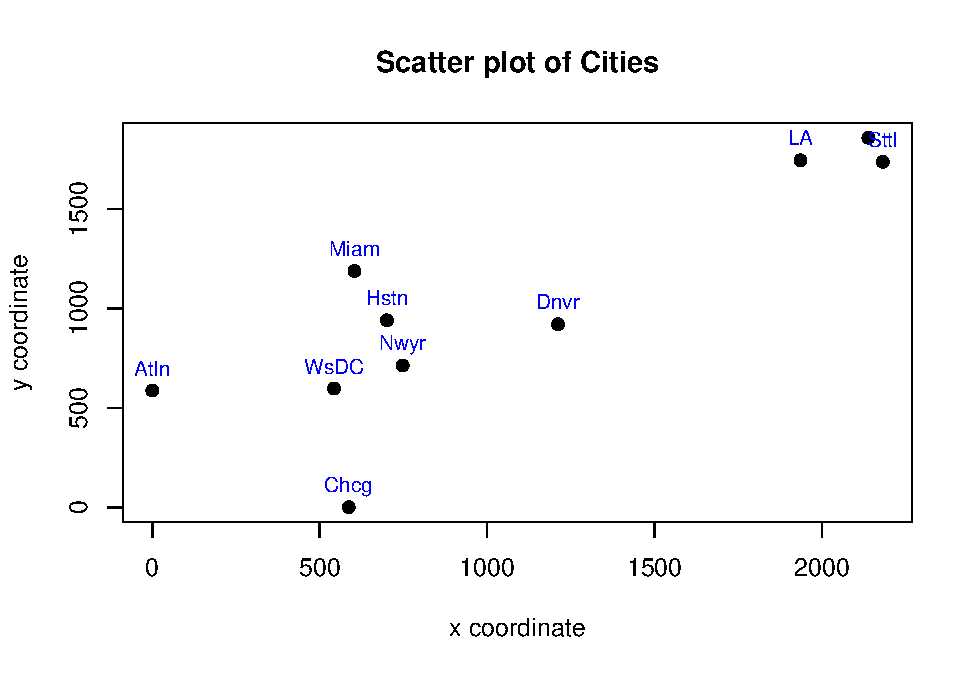
\includegraphics{hw7_files/figure-latex/unnamed-chunk-3-1.pdf}

\begin{quote}
\begin{enumerate}
\def\labelenumi{\arabic{enumi})}
\tightlist
\item
  Do the cluster analysis using (1) single linkage, (2) average linkage
  and (3) the centroid method.
\end{enumerate}
\end{quote}

(1)single linkage

\begin{Shaded}
\begin{Highlighting}[]
\NormalTok{hc1_cities<-}\KeywordTok{hclust}\NormalTok{(}\KeywordTok{dist}\NormalTok{(cities, }\DataTypeTok{method=}\StringTok{"euclidian"}\NormalTok{)^}\DecValTok{2}\NormalTok{, }\DataTypeTok{method=}\StringTok{"single"}\NormalTok{)}
\NormalTok{hc1_cities}
\end{Highlighting}
\end{Shaded}

\begin{verbatim}
## 
## Call:
## hclust(d = dist(cities, method = "euclidian")^2, method = "single")
## 
## Cluster method   : single 
## Distance         : euclidean 
## Number of objects: 10
\end{verbatim}

\begin{Shaded}
\begin{Highlighting}[]
\KeywordTok{rev}\NormalTok{(hc1_cities) }\CommentTok{#height : 군집간 거리 / merge: 병합순}
\end{Highlighting}
\end{Shaded}

\begin{verbatim}
## $dist.method
## [1] "euclidean"
## 
## $call
## hclust(d = dist(cities, method = "euclidian")^2, method = "single")
## 
## $method
## [1] "single"
## 
## $labels
##  [1] "Atlanta"      "Chicago"      "Denver"       "Houston"     
##  [5] "LA"           "Miami"        "Newyork"      "Sanfrancisco"
##  [9] "Seattle"      "WashingtonDC"
## 
## $order
##  [1]  9  5  8  3  4  6  7 10  1  2
## 
## $height
## [1]  272544  560711 1435040 1490187 1581207 2363192 2905270 4037129 4895001
## 
## $merge
##       [,1] [,2]
##  [1,]   -7  -10
##  [2,]   -5   -8
##  [3,]   -9    2
##  [4,]   -1   -2
##  [5,]    1    4
##  [6,]   -6    5
##  [7,]   -4    6
##  [8,]   -3    7
##  [9,]    3    8
\end{verbatim}


\end{document}
>>>>>>> 704346157696d5c879444e5bc135c15fa187d2e1
